% Caso de uso 1.4.3 -------------------------------------------------------------------------------
\begin{UseCase} {CU 1.4.3}{Eliminar proveedor}{
	Cambia el estado del proveedor seleccionado a suspendido (eliminación lógica).\label{CU: 1.4.3}
}

% Información del caso de uso ---------------------------------------------------------------------

\UCitem{Versión}{1.0}
\UCccsection{Administración}
\UCccitem{Autor}{Gonzaga Aparicio Josue}
\UCccitem{Evaluador}{}
\UCccitem{Operación}{}
\UCccitem{Prioridad}{Baja}
\UCccitem{Complejidad}{Baja}
\UCccitem{Volatilidad}{Baja}
\UCccitem{Madurez}{Alta}
\UCccitem{Estatus}{Finalizado}
\UCccitem{Fecha del último estatus}{20 de diciembre 2021}

% Revisión ----------------------------------------------------------------------------------------
% Copie y pegue este bloque tantas veces como revisiones tenga el caso de uso.
% Esta sección la debe llenar solo el Revisor

% Revisión Versión % Anote la versión que se revisó
\UCccsection{Revisión Versión 0.1 }

% Fecha % Anote la fecha en que se terminó la revisión
\UCccitem{Fecha}{} 

% Evaluador % Coloque el nombre completo de quien realizó la revisión
\UCccitem{Evaluador}{}

% Resultado % Coloque la palabra que mas se apegue al tipo de acción que el analista debe realizar
\UCccitem{Resultado}{}

% Observaciones % Liste los cambios que debe realizar el Analista.
\UCccitem{Observaciones}{}

% Atributos ---------------------------------------------------------------------------------------
	
\UCsection{Atributos}

	\UCitem{Actores}{
		{Empleado}.
	}

	\UCitem{Propósito}{
		Se hace con el fin de	evitar que aparezca en futuras busquedas.
	}

	\UCitem{Entradas}{
		
		\begin{UClist}			
			Datos necesarios para la busqueda:

			\UCli Empresa.
		\end{UClist}
	}

	\UCitem{Salidas}{
		Ninguna.
	}

	\UCitem{Precondiciones}{
		\begin{UClist}
			\UCli Debe existir el registro previo del proveedor.
		\end{UClist}
	}

	\UCitem{Postcondiciones}{
		Ninguna.
	}

	\UCitem{Reglas de negocio}{
		\begin{UClist}
			\UCli \cdtRef{RN-4}{RN-4 Proveedor pendiente}.
		\end{UClist}
	}

	\UCitem{Errores}{
		\begin{UClist}
			\UCli La base de datos puede estar caída.
			\UCli Es posible que no haya proveedores registrados.
		\end{UClist}
	}

	\UCitem{Tipo}{
		
	}
\end{UseCase}

%Trayectoria principal ----------------------------------------------------------------------------

\begin{UCtrayectoria}

	\UCpaso [\UCactor]	Selecciona \cdtButton{Proveedores} en el la interfaz Menu principal. Consultar en página: \ref{UI: menu principal} 	\label{CU 1.4.3:P1}
	\UCpaso [\UCsist]		Muestra la interfaz Gestionar proveedor.  \label{CU 1.4.3:P2}
	\UCpaso [\UCsist]		Obtiene todos los datos de los proveedores de la BD. \refTray{A}
	\UCpaso [\UCsist]		Muestra la interfaz Gestionar proveedor con los datos anteriores. Consultar en página: \ref{UI: gestionar proveedor} \label{CU 1.4.3:P4}
	\UCpaso [\UCactor]	Selecciona el icono \btnBorrar del proveedor que quiere eliminar.\refTray{B}\label{CU 1.4.3:P5}
	\UCpaso [\UCsist]		Muestra mensaje: ¿Seguro que quiere eliminar al proveedor?. Consultar en página: \ref{UI: confirmar eliminar}
	\UCpaso [\UCactor]	Selecciona \cdtButton{Si}. \refTray{C} \refTray{D}
	\UCpaso [\UCsist]		Cambia el estado del proveedor a suspendido en la base de datos, a corde al diagrama DE Proveedor \refTray{B}
	\UCpaso [\UCsist]		Muestra mensaje: El proveedor fue borrado con éxito. Consultar en página: \ref{UI: exito al eliminar}
	\UCpaso [\UCactor]	Selecciona \cdtButton{OK}
	\UCpaso [\UCsist]		Muestra la interfaz Gestionar proveedor. Consultar en página: \ref{UI: gestionar proveedor}

\end{UCtrayectoria}


% Trayectorias alternativas -----------------------------------------------------------------------
{
% Trayectoria A
%\begin{UCtrayectoriaA}{A}{Sin proveedores previamente registrados}
%	\UCpaso [\UCsist]		Muestra mensaje: \cdtRef{MSG}{No hay proveedores registrados}.
%	\UCpaso [\UCactor]	Selecciona \cdtButton{OK}
%	\UCpaso Regresa al paso \ref{CU 1.4.3:P4} de la trayectoria principal.
%\end{UCtrayectoriaA}

% Trayectoria B
\begin{UCtrayectoriaA}{A}{Base de datos no disponible}
	\UCpaso [\UCsist]		Muestra mensaje: "Base de Datos no disponible, por favor intente más tarde".
	\UCpaso [\UCactor]	Selecciona \cdtButton{OK}
	\UCpaso Muestra la interfaz Menu principal. Consultar en página: \pageref{UI: menu principal}
\end{UCtrayectoriaA}

% Trayectoria C
\begin{UCtrayectoriaA}{B}{Busca el proveedor que quiere borrar}
	\UCpaso Include: \cdtRef{CU 1.4.2}{CU 1.4.2 Consultar proveedor}.
	\UCpaso Regresa al paso \ref{CU 1.4.3:P5} de la trayectoria principal.
\end{UCtrayectoriaA}

% Trayectoria E
\begin{UCtrayectoriaA}{C}{Selecciona No}
	\UCpaso [\UCactor]	Selecciona \cdtButton{No}
	\UCpaso Regresa al paso \ref{CU 1.4.3:P2} de la trayectoria principal.
\end{UCtrayectoriaA}

% Trayectoria F
\begin{UCtrayectoriaA}{D}{Incumplimiento de la RN Provedor con pedido pendiente}
	\UCpaso [\UCsist]		Muestra mensaje: "El proveedor cuenta con pedido pendiente, no puede ser borrado".
	\UCpaso Regresa al paso \ref{CU 1.4.3:P2} de la trayectoria principal.
\end{UCtrayectoriaA}

}
{
\begin{flushleft}
	\break
	% Clases
	\Large{Clases}\\
	\rule{14cm}{0.5pt}

	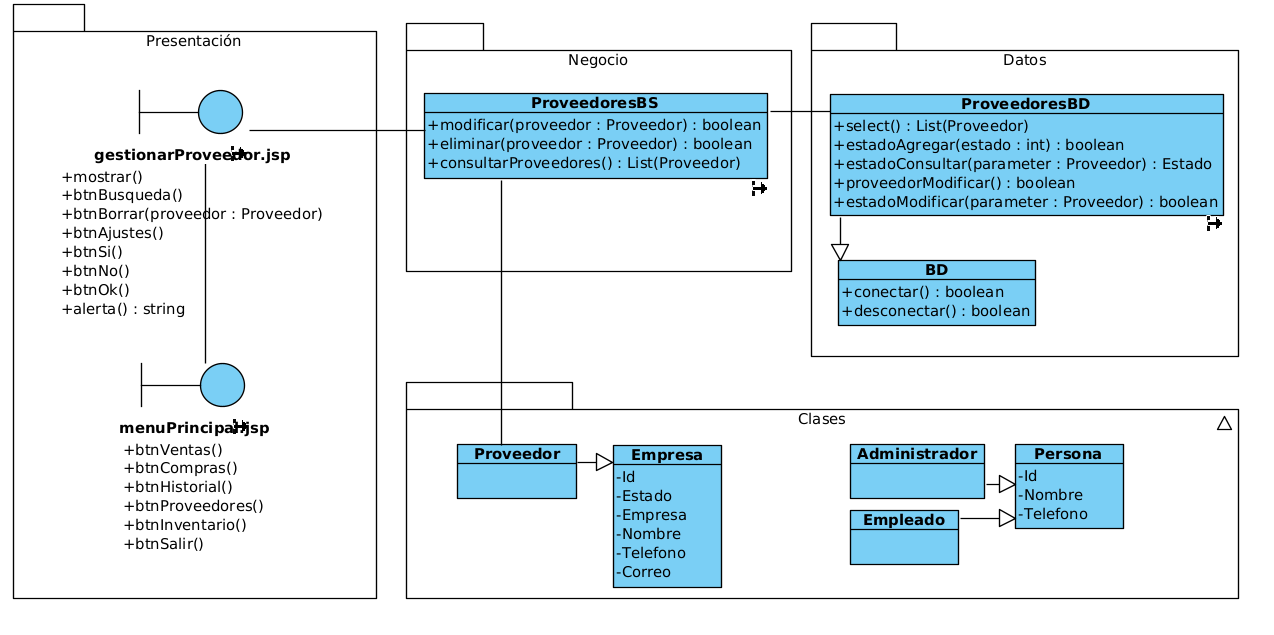
\includegraphics[height=8cm]{casouso/cu1.4.3/images/clases.png}\\	

	% Secuencia
	\Large{Secuencia}\\
	\rule{14cm}{0.5pt}

	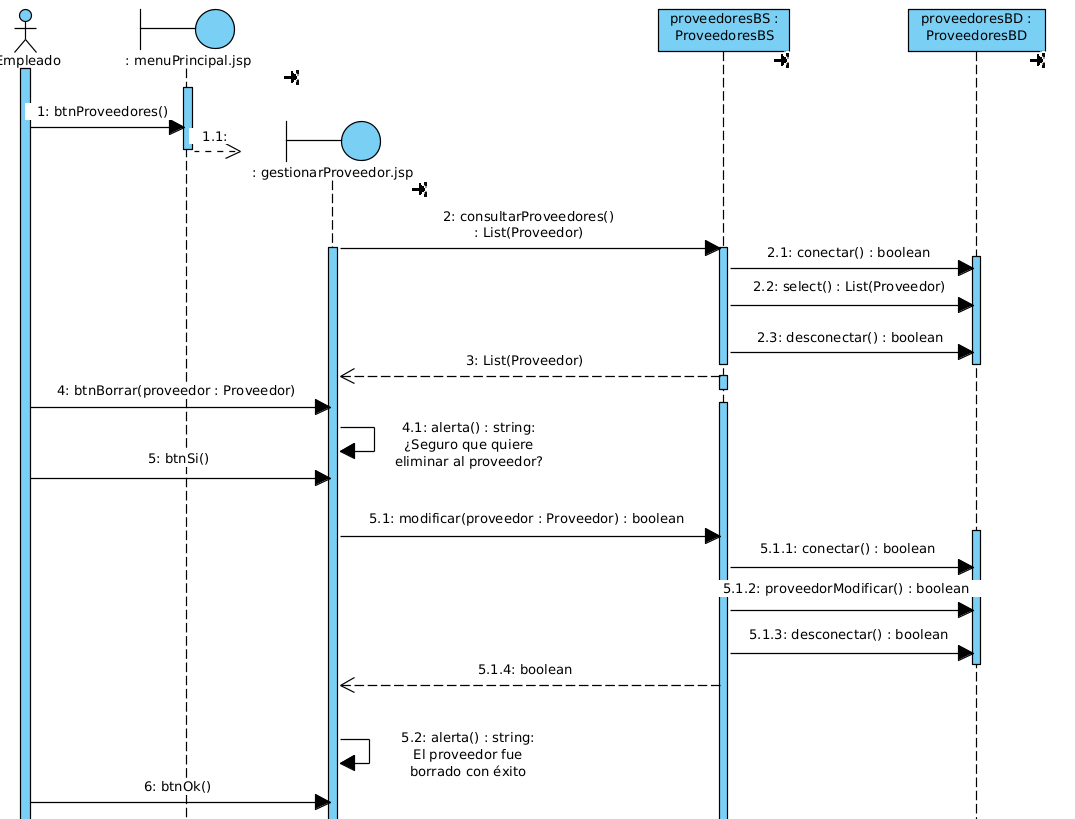
\includegraphics[height=10cm]{casouso/cu1.4.3/images/secuencia.png}\\	
	
\end{flushleft}
}